\chapter{C:简化功能点 (SiFP)练习题} % Introduction chapter suppressed from the table of contents

\hypertarget{ux65c5ux6e38ux670dux52a1-ux5f00ux53d1ux9879ux76eetourist-services---development-project}{%
\subsection{3.旅游服务-开发项目Tourist Services - Development
Project}\label{ux65c5ux6e38ux670dux52a1-ux5f00ux53d1ux9879ux76eetourist-services---development-project}}

\hypertarget{description}{%
\subsubsection{Description}\label{description}}

Wonder
Travel公司计划将其行程(Trips)管理系统自动化,该系统将连接各旅行预订系统
(travel Booking systems) 和行程路线(PV)系统。\\

\hypertarget{functional-requirements}{%
\subsubsection{Functional requirements}\label{functional-requirements}}

该系统将由基于菜单界面的在线组件和定期运行的批处理组件组成。\\

\hypertarget{rf01}{%
\paragraph{RF01}\label{rf01}}

将使用行程包的行程码(ID)作为索引,存储数据。\\
行程(Trips)包括:

\begin{itemize}
\tightlist
\item
  行程码(ID)
\item
  行程路线编号(PV)
\item
  符合资格的导游姓名
\item
  行程类型(汽车、巴士、火车、飞机、游轮、混合)
\item
  计划版本数
\item
  版本频次(月、季等)\\
\end{itemize}

用户将从下拉列表中选择行程路线编号(PV code)
(来自行程路线(PV)文件),系统会 自动生成行程码 (Trip code)。 行程路线
Trip Routes (PV)
文件包含旅游区域(例如:北欧、北极、突尼斯、土耳其、希腊、美国、古巴和加勒比地区、日本、中国、埃及\ldots{}\ldots{}等等,信息都是由外部系统管理。\\
从导游注册文件中获得有资格的导游的名字,然后利用下拉列表来设置哪位导游有资格带哪个行程(Trip)。\\
版本状态字段将自动设置为``planned''(已策划)\\
行程类型将通过一个下拉列表来设置一些值,如``文化''或``休闲''或``宗教''等
使用功能键 (function
key)完成验证、一致性检查(编辑)和写入输入的数据,系统会按需要报错。\\

\hypertarget{rf02}{%
\paragraph{RF02}\label{rf02}}

基于行程码(ID) (Trip code) 和功能键选择 Trips\\
Trips将显示与上一段中包含的相同数据,以及从PV文件中提取的数据,以及从RF07段中提到的导游注册文件中提取的导游的详细数据。\\
与前一节相同的Trips下拉列表将用于帮助用户进行选择。\\
如果trip文件中不存在搜索的行程码(ID),系统将报错。\\

\hypertarget{rf03}{%
\paragraph{RF03}\label{rf03}}

RF01中包含的所有字段都可以修改 - 除了行程码(ID)(因为它是作为索引)。\\
版本状态字段只能通过 选择下拉列表中来更改, 只可以更改 包含``已提供
provided''和``已删除 deleted''值的内容。\\
无论如何,如更新版本状态字段将会自动更新:\\
* 余下可提供的版本数\#\#\\
::(\#\# 计划可提供版本数,减去已提供/删除的版本数)\\
也可用与RF01中相同的导游下拉列表挑选导游。\\
使用功能键 (function
key)完成验证、一致性检查(编辑)和写入输入的数据,系统会按需要报错。\\

\hypertarget{rf04}{%
\paragraph{RF04}\label{rf04}}

选择行程码,按下功能键,即可取消行程。\\
使用RF01中提到相同下拉列表,来选择要删除的行程。如果Trip文件中不存在该行程码(ID),系统将报错。\\
也有取消确认消息。\\

\hypertarget{rf05}{%
\paragraph{RF05}\label{rf05}}

用户将能够查看属于某个行程路线(PV)的旅行版本的信息。用户必须输入行程码(ID)(Trip
code) 并按下功能键。选择的行程版本将显示以下数据:\\
*行程码(ID)

\begin{itemize}
\tightlist
\item
  行程描述
\item
  PV号
\item
  PV描述
\item
  导游姓名(所有符合资格的导游)
\item
  导游资格(所有有资格参加本次旅行的导游)
\item
  计划的版本数
\item
  版本的频率
\item
  提供的版本数
\item
  每个版:

  \begin{itemize}
  \tightlist
  \item
    版ID
  \item
    版日期
  \item
    版状态(已计划/提供/删除)
  \item
    已选择的导游\\
  \end{itemize}
\end{itemize}

行程描述和PV描述数据是从PV文件中提取。 用户也可以要求打印显示的信息。\\

\hypertarget{rf06}{%
\paragraph{RF06}\label{rf06}}

由于WonderTravel提供的旅行具有季节性,通过选择行程代码(必须存在于旅行文件中)并输入版本日期(必须大于第一次输入的版本日期)来生成行程的版本。系统会自动生成唯一的版本码。版本的日期考虑了季节性相关的选择。\\
版本状态字段会自动设置为``planned''。一个功能键将激活数据的写入。如果需要,将生成错误消息。\\

\hypertarget{rf07}{%
\paragraph{RF07}\label{rf07}}

有关导游的信息将以导游的姓名作为索引保存在导游登记簿中。\\

\hypertarget{rf08}{%
\paragraph{RF08}\label{rf08}}

使用导游的姓名和功能键选择 ,
便可以显示导游信息。如果导游登记簿指南中不存在该导游,系统将生成一条消息。下拉列表与RF01的导游下拉列表相同。\\

\hypertarget{rf09}{%
\paragraph{RF09}\label{rf09}}

除了导游的名称(因为它是索引),导游数据都可以更改。\\
可用于与RF01段相同的导游下拉列表,选择要修改数据的导游。\\
使用功能键 (function
key)完成验证、一致性检查(编辑)和写入输入的数据,系统会按需要报错。\\

\hypertarget{rf10}{%
\paragraph{RF10}\label{rf10}}

输入的旅行文件数据将通过一个文件发送到后台预订系统,更新 行程(Trips)
。信息来自行程(Trips) 文档及导游登记册(Guides Register) 。\\
%\href{文件:Sifp_3_1.png}{文件:Sifp 3 1.png}

%\href{文件:Sifp_3_2.png}{文件:Sifp 3 2.png}

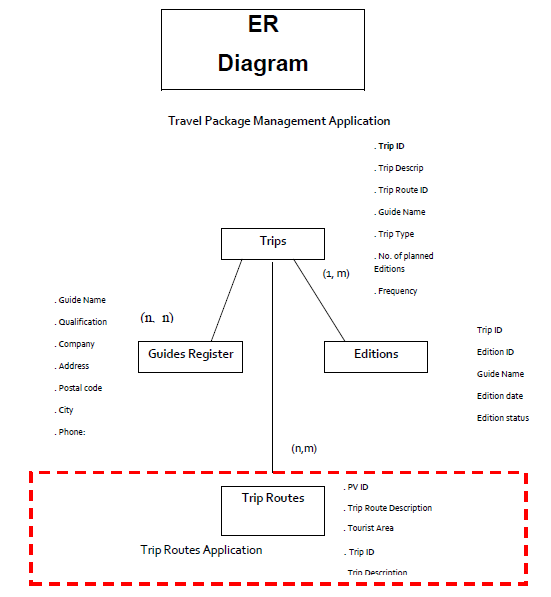
\includegraphics[width=6cm]{Sifp_3_1.png}

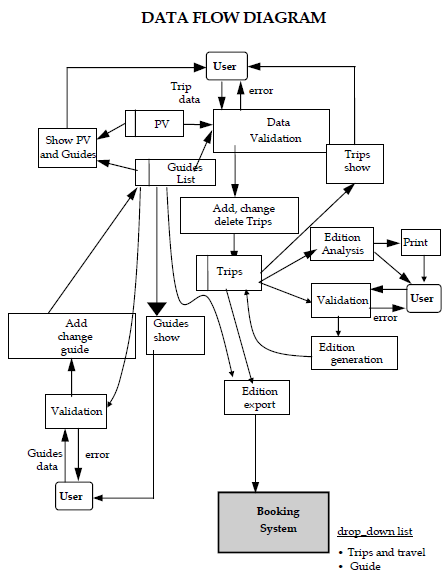
\includegraphics[width=6cm]{Sifp_3_2.png}

\hypertarget{ux65c5ux6e38ux670dux52a1--femux9879ux76ee-tourist-services-fem-project}{%
\subsection{4.旅游服务- FEM项目 Tourist Services -- FEM
Project}\label{ux65c5ux6e38ux670dux52a1--femux9879ux76ee-tourist-services-fem-project}}

\hypertarget{description-1}{%
\subsubsection{Description}\label{description-1}}

基于以上例子3的旅游服务系统的基础上,提出以下软件功能增强与维护(FEM)\\

\hypertarget{functional-requirements-1}{%
\subsubsection{Functional
requirements}\label{functional-requirements-1}}

\hypertarget{rf01-1}{%
\subsubsection{RF01}\label{rf01-1}}

功能增强维护后,行程(Trips)管理系统必须显示在PV文件中旅行国家的当前政治局势的信息。\\

\hypertarget{rf02-1}{%
\subsubsection{RF02}\label{rf02-1}}

有关导游经验的信息必须在导游登记档案的旅游领域(tourism)中处理。\\


\hypertarget{rf03-1}{%
\subsubsection{RF03}\label{rf03-1}}

必须提供用户最多选择的行程/旅行套餐的统计数据。\\

\hypertarget{rf04-1}{%
\subsubsection{RF04}\label{rf04-1}}

行程/旅游套餐必须送到相关政府部门备案。\\


